\section{Results}
\label{sec:results}
Unless stated otherwise, the local hit probability is 20\%, the switch cost is 0.02~$\mu$s and all values come from the seed-42 runs described in Section~\ref{sec:method}. Latencies are in microseconds.

\subsection{Throughput under increasing load}
Figure~\ref{fig:tput} plots the carried throughput against the offered load. Up to 1.5~MRPS every policy carries the whole load. At 1.8~MRPS the busy-wait system already falls slightly short (1.77~MRPS) while the yield systems still carry 1.80. From there the curves separate. Busy-wait stays at 1.77~MRPS however much load is offered, which is 97.7\% of its bound $\Lambda_{bw}=1.81$~MRPS from Equation~\eqref{eq:lbw}. Yield follows the offered load up to 2.5~MRPS and then stays at 2.50~MRPS, which is its link bound from Equation~\eqref{eq:llink} to within 0.1\%. The ratio of the two plateaus is $2.497/1.772=1.41$. The two dispatch rules give identical throughput.

\begin{figure}[t]
\centering
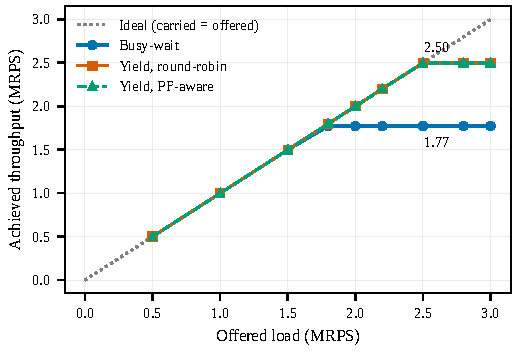
\includegraphics[width=\columnwidth]{tput}
\caption{Carried throughput against offered load for the three policies. The dotted line shows carried equal to offered.}
\label{fig:tput}
\end{figure}

\subsection{Tail latency}
Figure~\ref{fig:p999} shows the 99.9th percentile of latency, and Table~\ref{tab:main} gives the full set of percentiles. At 0.5~MRPS the policies are indistinguishable (6.5 and 6.6~$\mu$s at P99.9), and the median is 5.30 versus 5.32~$\mu$s, a difference of 0.02~$\mu$s that comes from the two extra switches of a miss. As the load rises, the busy-wait tail grows first. At 1.0~MRPS the P99.9 is 8.7~$\mu$s against 7.7 for yield. At 1.5~MRPS it is 17.2 against 8.9~$\mu$s, a factor of 1.93, and the P99 is 13.1 against 7.8~$\mu$s (1.68). At 1.8~MRPS busy-wait is past its capacity and the P99.9 jumps to about 3{,}000~$\mu$s, while yield has 10.6~$\mu$s. If a service-level target of 20~$\mu$s at P99.9 is assumed, busy-wait can carry about 1.5~MRPS (26.7~$\mu$s at 1.6) and yield about 2.2~MRPS (18.1~$\mu$s), a factor of roughly 1.5 in usable load.

\begin{figure}[t]
\centering
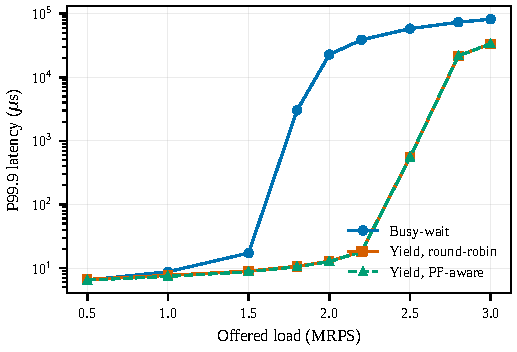
\includegraphics[width=\columnwidth]{p999}
\caption{99.9th percentile latency against offered load (log scale). Values above each policy's capacity understate the true delay (Section~\ref{sec:method}).}
\label{fig:p999}
\end{figure}

\begin{figure}[t]
\centering
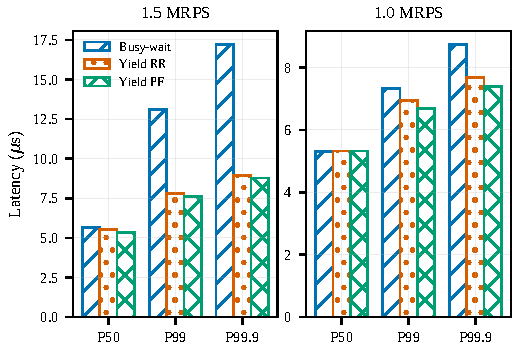
\includegraphics[width=\columnwidth]{bars}
\caption{Latency percentiles of the three policies at 1.0 and 1.5~MRPS.}
\label{fig:bars}
\end{figure}

The yield system keeps its P99.9 under 20~$\mu$s until 2.2~MRPS and reaches 552~$\mu$s at 2.5~MRPS, the load at which the link is exactly full. Above 2.5~MRPS both policies are overloaded and their latencies depend on how long the run lasts, so they are not comparable results. The PF-aware variant is almost the same as round-robin here (8.8 against 8.9~$\mu$s at 1.5~MRPS), which Section~\ref{sec:pf} examines.

\begin{table*}[t]
\caption{Throughput (MRPS) and latency ($\mu$s) of the three policies. The last column is the P99.9 of the PF-aware yield system.}
\label{tab:main}
\centering
\footnotesize
\begin{tabular}{r|rrrr|rrrr|r}
\toprule
 & \multicolumn{4}{c|}{Busy-wait} & \multicolumn{4}{c|}{Yield, round-robin} & PF-aware \\
Offered & Tput & P50 & P99 & P99.9 & Tput & P50 & P99 & P99.9 & P99.9 \\
\midrule
0.5 & 0.50 & 5.3 & 6.0 & 6.5 & 0.50 & 5.3 & 6.1 & 6.6 & 6.5 \\
1.0 & 1.00 & 5.3 & 7.3 & 8.7 & 1.00 & 5.3 & 6.9 & 7.7 & 7.4 \\
1.5 & 1.50 & 5.7 & 13.1 & 17.2 & 1.50 & 5.5 & 7.8 & 8.9 & 8.8 \\
1.8 & 1.77 & 1{,}626.7 & 2{,}948.4 & 3{,}014.3 & 1.80 & 5.8 & 9.0 & 10.6 & 10.5 \\
2.0 & 1.77 & 12{,}597.8 & 22{,}470.9 & 22{,}685.0 & 2.00 & 6.0 & 10.4 & 12.8 & 12.7 \\
2.2 & 1.77 & 21{,}786.2 & 38{,}449.5 & 38{,}787.7 & 2.20 & 6.4 & 13.9 & 18.1 & 18.0 \\
2.5 & 1.77 & 33{,}194.4 & 57{,}631.3 & 58{,}113.1 & 2.50 & 94.2 & 536.0 & 551.8 & 551.8 \\
2.8 & 1.77 & 42{,}476.4 & 72{,}710.2 & 73{,}297.4 & 2.50 & 11{,}460.3 & 21{,}461.4 & 21{,}708.8 & 21{,}708.7 \\
3.0 & 1.77 & 47{,}802.0 & 81{,}094.1 & 81{,}733.1 & 2.50 & 18{,}238.9 & 33{,}217.5 & 33{,}580.3 & 33{,}580.3
\\
\bottomrule
\end{tabular}
\end{table*}

\subsection{Effect of the local hit rate}
\label{sec:hit}
Figure~\ref{fig:hit} and Table~\ref{tab:hit} show the peak throughput when the local hit rate varies from 10\% to 80\%. The offered load is 4.0~MRPS, so any value equal to 4.0 is a lower bound. For hit rates where neither system is capped the ratio of yield to busy-wait is 1.37 at 10\%, 1.41 at 20\% and 1.51 at 40\%. It is therefore not largest at low hit rates, which is where a first reading of the argument for yielding might place it. The bound ratio explains why: the yield ceiling $1/((1-h)t_\ell)$ and the busy-wait ceiling $N/S_{bw}$ both rise as $h$ grows, but the second rises more slowly while it is not yet limited by the processors. At 60\% the yield system is cut off by the offered load (4.0 against a bound of 5.0), so the measured ratio of 1.35 is only a lower bound; the bounds themselves give 5.00/3.04, about 1.64. At 80\% both systems reach the offered load and show no difference.

\begin{figure}[t]
\centering
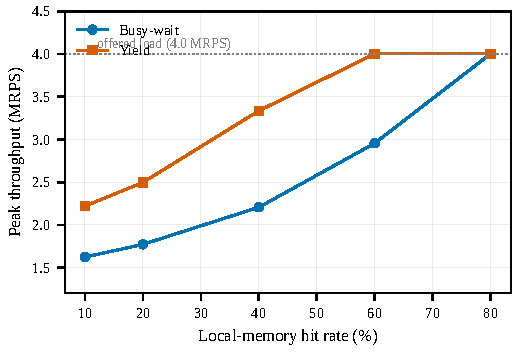
\includegraphics[width=\columnwidth]{hit}
\caption{Peak throughput against the local hit rate, with an offered load of 4.0~MRPS.}
\label{fig:hit}
\end{figure}

\begin{table}[t]
\caption{Hit-rate sweep: analytic bound and measured peak (MRPS). $^{\dagger}$ capped by the offered load of 4.0~MRPS.}
\label{tab:hit}
\centering
\footnotesize
\setlength{\tabcolsep}{3pt}
\begin{tabular}{r|rrr|rrr|r}
\toprule
 & \multicolumn{3}{c|}{Busy-wait} & \multicolumn{3}{c|}{Yield} & Ratio \\
$h$ (\%) & Bound & Meas. & \% & Bound & Meas. & \% & Y/B \\
\midrule
10 & 1.648 & 1.623 & 98.5 & 2.222 & 2.220 & 99.9 & 1.37 \\
20 & 1.814 & 1.772 & 97.7 & 2.500 & 2.497 & 99.9 & 1.41 \\
40 & 2.273 & 2.206 & 97.1 & 3.333 & 3.336 & 100.1 & 1.51 \\
60 & 3.042 & 2.956 & 97.2 & 4.000$^{\dagger}$ & 4.003 & 100.1 & $\geq$1.35 \\
80 & 4.000$^{\dagger}$ & 4.004 & 100.1 & 4.000$^{\dagger}$ & 4.003 & 100.1 & 1.00$^{\dagger}$
\\
\bottomrule
\end{tabular}
\end{table}

The column marked ``\%'' compares measurement with bound. For busy-wait the measured peak is 97.1--98.5\% of the bound in all uncapped rows, with the shortfall caused by queueing in the link, and for yield it is 99.9--100.1\%. The simple formulas of Section~\ref{sec:bounds} therefore describe the simulator well.

In the Adios paper, reducing local memory from the full working set down to a tenth of it costs the yield-based system 25\% of its throughput and the busy-wait system 60\% \cite{adios}. Our model does not reproduce that pattern. Between 40\% and 10\% hit rate the busy-wait peak falls by 26\% (2.21 to 1.62) and the yield peak by 33\% (3.34 to 2.22), because the link ceiling of the yield system is inversely proportional to the miss rate. The offered-load cap prevents a comparison over the paper's full range, so we make no claim about the 100\%--10\% interval.

\subsection{Page-fault-aware dispatch}
\label{sec:pf}
Table~\ref{tab:pf} and Figure~\ref{fig:pfgain} compare the P99.9 latency of the two dispatch rules, averaged over five seeds, at loads between 1.8 and 2.4~MRPS and for both queue-pair settings. The PF-aware rule is better at nine of the ten points, by 0.09\% to 1.22\%, with an average gain of 0.61\% for $t_q=1$~$\mu$s and 0.51\% for $t_q=2$~$\mu$s. The gain is largest at the lowest load tested and shrinks as the load approaches the link limit; at 2.4~MRPS with $t_q=2$~$\mu$s the sign reverses ($-0.12$\%), which is the size of the noise in these runs.

\begin{table}[t]
\caption{P99.9 latency ($\mu$s, mean of five seeds) of round-robin (RR) and PF-aware dispatch.}
\label{tab:pf}
\centering
\footnotesize
\begin{tabular}{llrrr}
\toprule
Setting & Load & RR & PF & Gain (\%) \\
\midrule
QP 1.0 & 1.8 & 10.87 & 10.73 & +1.22 \\
QP 1.0 & 2.0 & 13.28 & 13.17 & +0.81 \\
QP 1.0 & 2.2 & 18.60 & 18.50 & +0.57 \\
QP 1.0 & 2.3 & 25.20 & 25.11 & +0.37 \\
QP 1.0 & 2.4 & 42.86 & 42.82 & +0.09 \\
QP 2.0 & 1.8 & 10.95 & 10.83 & +1.17 \\
QP 2.0 & 2.0 & 13.36 & 13.26 & +0.78 \\
QP 2.0 & 2.2 & 18.61 & 18.55 & +0.32 \\
QP 2.0 & 2.3 & 25.22 & 25.12 & +0.42 \\
QP 2.0 & 2.4 & 42.85 & 42.90 & -0.12
\\
\bottomrule
\end{tabular}
\end{table}

\begin{figure}[t]
\centering
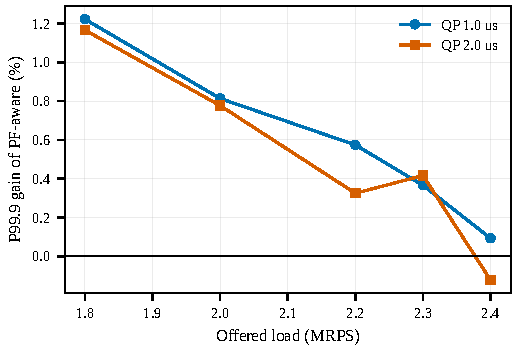
\includegraphics[width=\columnwidth]{pfgain}
\caption{Gain of PF-aware over round-robin dispatch in P99.9 latency, in percent.}
\label{fig:pfgain}
\end{figure}

The published gain is larger: up to 7.5\% for Memcached and 27\% for RocksDB \cite{adios}. A likely reason for the difference follows from the model. At 2.5~MRPS each queue pair handles 0.25 fetches per microsecond, which keeps it 25\% busy for $t_q=1$ and 50\% busy for $t_q=2$, while the shared link is 100\% busy. The dispatcher can move fetches between queue pairs but cannot reduce the load on the link, so the delay that it could remove is small. Real queue pairs have burstier arrivals and variable service times, which our fixed-time model lacks. We have not tested this explanation with a modified model, so it is a hypothesis.

\subsection{Cost of a context switch}
\label{sec:switch}
Figure~\ref{fig:switch} and Table~\ref{tab:switch} vary the cost $t_s$ of one switch from 0.02 to 4~$\mu$s. For $t_s\le0.5$~$\mu$s the yield peak is 2.50~MRPS, the link bound, because the processors still have spare capacity. For larger costs the processors become the bottleneck and the peak follows $\Lambda_{cpu}$, falling to 2.21 at 1~$\mu$s, 1.81 at 1.5~$\mu$s and 0.95~MRPS at 4~$\mu$s. By linear interpolation the throughput of yield and busy-wait are equal at $t_s\approx1.57$~$\mu$s, which agrees with the break-even rule $t_s<t_f/2=1.5$~$\mu$s of Equation~\eqref{eq:breakeven} (the small excess comes from the 2.3\% by which the real busy-wait plateau lies under its bound). For the tail at 1.5~MRPS, yield stays below busy-wait's 17.2~$\mu$s up to about 1.44~$\mu$s.

Both reported switch costs for user-level threads---0.02~$\mu$s (40 cycles) for Adios's unithreads and 0.10~$\mu$s (191 cycles) for Shinjuku \cite{adios}---fall comfortably below this 1.5~$\mu$s ceiling. In contrast, standard kernel-space context switching takes $\approx 4~\mu$s \cite{adios}, driving yield capacity down to 0.95~MRPS (merely 54\% of spinning throughput). This confirms the paper's core thesis: yielding's feasibility in disaggregated paging hinges entirely on keeping thread-switch overhead below microsecond scales.

\begin{figure*}[t]
\centering
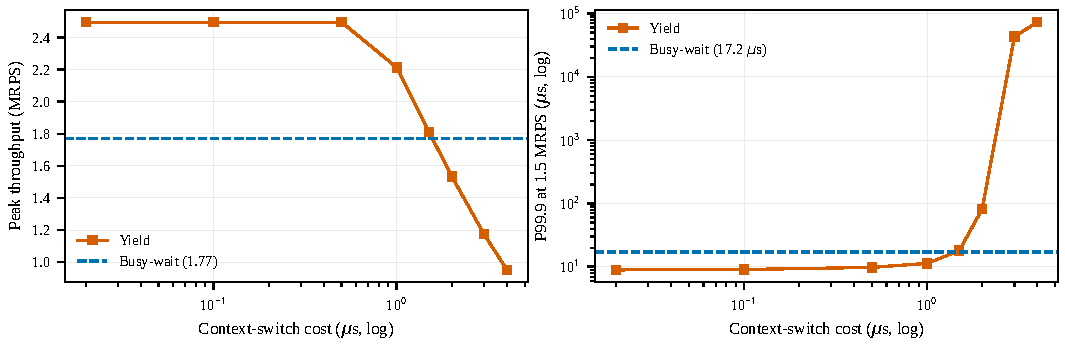
\includegraphics[width=0.92\textwidth]{switch}
\caption{Effect of the context-switch cost on the yield system. Left: peak throughput. Right: P99.9 latency at 1.5~MRPS. Dashed lines show busy-wait.}
\label{fig:switch}
\end{figure*}

\begin{table}[t]
\caption{Switch-cost sweep: analytic yield bound and measured peak (MRPS), and P99.9 at 1.5~MRPS ($\mu$s).}
\label{tab:switch}
\centering
\footnotesize
\begin{tabular}{rrrrr}
\toprule
$t_s$ ($\mu$s) & Bound & Meas. & \% & P99.9 \\
\midrule
0.02 & 2.500 & 2.497 & 99.9 & 8.9 \\
0.1 & 2.500 & 2.497 & 99.9 & 9.1 \\
0.5 & 2.500 & 2.497 & 99.9 & 9.8 \\
1 & 2.216 & 2.214 & 99.9 & 11.3 \\
1.5 & 1.814 & 1.813 & 99.9 & 18.0 \\
2 & 1.536 & 1.535 & 100.0 & 82.0 \\
3 & 1.175 & 1.174 & 99.9 & 43133.5 \\
4 & 0.951 & 0.951 & 100.0 & 73011.6
\\
\bottomrule
\end{tabular}
\end{table}

\subsection{Realistic hit rates: LRU cache and skewed access}
\label{sec:cache}
The fixed 20\% hit probability is a simplification, since real hit rates come from cache size and access skew. Table~\ref{tab:cache} reports the LRU model of Section~\ref{sec:model} with an offered load of 5.0~MRPS. First, uniform access ($s=0$) with a 20\% cache produces a hit rate of 19.9\% and the same throughputs as the fixed model (1.77 and 2.50~MRPS), which validates the shortcut. Second, skew raises the hit rate sharply: 31.8\% at $s=0.5$, 59.3\% at $s=0.8$ and 80.6\% at $s=0.99$. With it both throughputs rise and the ratio grows from 1.41 to 1.67 at a hit rate of 59\%. This matches the 1.64 predicted from the bounds at the same hit rate (5.0/3.04 is the bound ratio at 60\%) and agrees with the corresponding row of the hit-rate sweep. Third, a larger cache has the same effect as more skew (Figure~\ref{fig:cache}): at $s=0.8$ the yield peak grows from 3.08 to 4.87~MRPS as the cache grows from 5\% to 20\% of the pages. Rows marked $^{\ddagger}$ equal the offered load and carry no ratio.

\begin{table}[t]
\caption{LRU cache with Zipf access: hit rate and peak throughput (MRPS). $^{\ddagger}$ equals the offered load of 5.0~MRPS (read as ``at least'').}
\label{tab:cache}
\centering
\footnotesize
\begin{tabular}{rrrrr}
\toprule
Skew / size & Hit (\%) & Busy-wait & Yield & Ratio \\
\midrule
\multicolumn{5}{l}{\textit{Skew sweep (cache 20\%)}} \\
0 & 19.9 & 1.77 & 2.50 & 1.41 \\
0.5 & 31.8 & 2.00 & 2.90 & 1.45 \\
0.8 & 59.3 & 2.92 & 4.87 & 1.67 \\
0.99 & 80.6 & 4.56 & 5.01$^{\ddagger}$ & $\geq$1.10 \\
1.2 & 94.8 & 5.01$^{\ddagger}$ & 5.01$^{\ddagger}$ & -- \\
\multicolumn{5}{l}{\textit{Size sweep (skew 0.8)}} \\
5\% & 36.2 & 2.12 & 3.08 & 1.45 \\
10\% & 46.5 & 2.41 & 3.68 & 1.53 \\
20\% & 59.3 & 2.92 & 4.87 & 1.67 \\
40\% & 75.2 & 3.96 & 5.01$^{\ddagger}$ & $\geq$1.26 \\
60\% & 85.9 & 5.01$^{\ddagger}$ & 5.01$^{\ddagger}$ & --
\\
\bottomrule
\end{tabular}
\end{table}

\begin{figure*}[t]
\centering
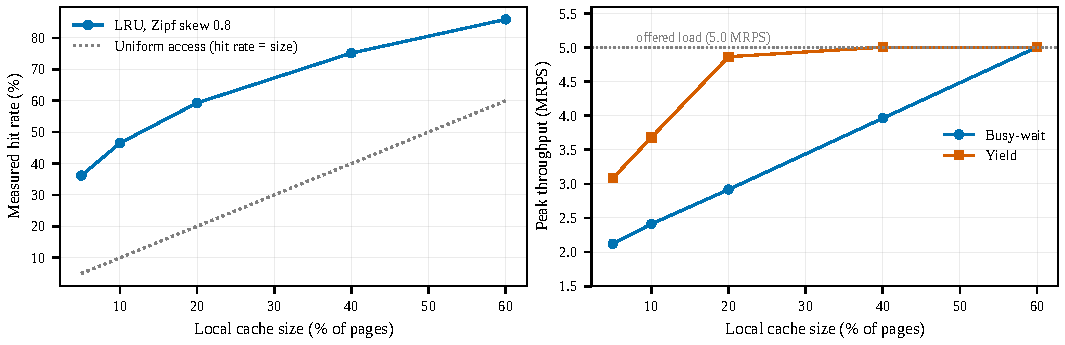
\includegraphics[width=0.92\textwidth]{cache}
\caption{LRU cache with Zipf skew 0.8. Left: measured hit rate against cache size. Right: peak throughput against cache size.}
\label{fig:cache}
\end{figure*}

\begin{figure}[t]
\centering
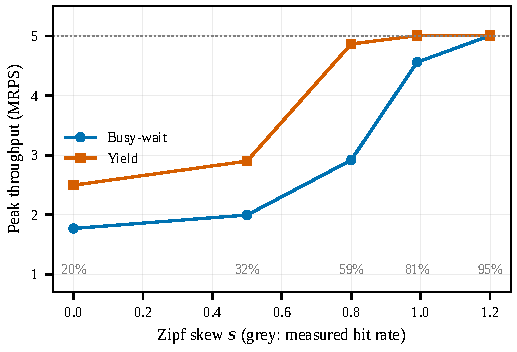
\includegraphics[width=\columnwidth]{skew}
\caption{Peak throughput against Zipf skew for a 20\% cache. Grey numbers are the measured hit rates.}
\label{fig:skew}
\end{figure}

\subsection{Load-Aware Adaptive Hybrid Yielding}
\label{sec:adaptive}
Evaluating pure spinning against pure yielding exposes an inherent tension across load regimes. Under light traffic ($< 1.0$~MRPS), processor cores sit idle between request arrivals. Unconditionally yielding on every miss forces the system to pay a 40~ns round-trip context-switch penalty ($2 \times 0.02~\mu$s) even though no other task is waiting for the CPU, giving busy-waiting a slight latency edge (5.30~$\mu$s vs.\ 5.32~$\mu$s median). If thread switches are slower ($t_s \ge 0.5~\mu$s), this light-load penalty swells to 28\% at $t_s = 1.5~\mu$s. Conversely, under heavy traffic ($> 1.5$~MRPS), spinning suffers from severe HOL blocking: worker cores stall waiting on RDMA packets, capping throughput at 1.77~MRPS and causing tail latency ($P_{99.9}$) to jump from 17.2~$\mu$s to over 3{,}000~$\mu$s.

To resolve this dilemma, we evaluate our \emph{Load-Aware Adaptive Hybrid Yielding} policy (\texttt{sweep\_adaptive.py}). Workers consult the local condition in Equation~\eqref{eq:must_yield} during fault handling: if work is queued locally, in the central dispatcher, or if peer cores are saturated, the worker yields immediately to prevent blocking. Otherwise, it polls locally on the RDMA completion queue.

\begin{figure*}[t]
\centering
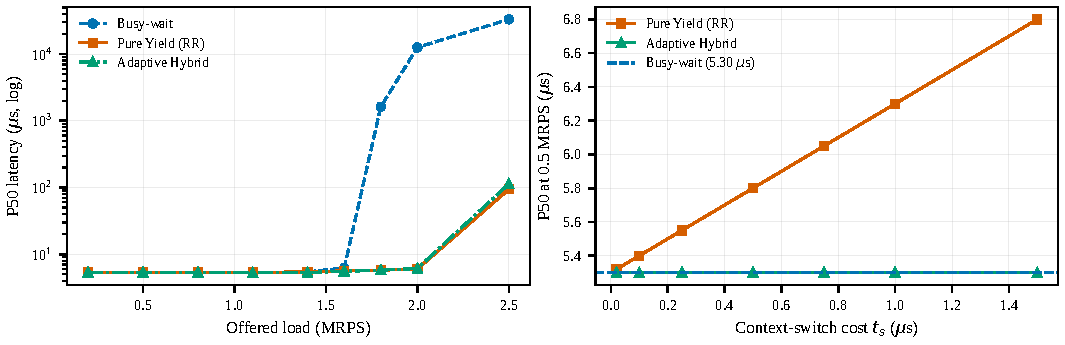
\includegraphics[width=0.92\textwidth]{adaptive}
\caption{Performance of the Load-Aware Adaptive Hybrid Yielding strategy. Left: median latency ($P_{50}$) across offered loads (0.2--2.5~MRPS). Right: sensitivity of median latency ($P_{50}$) to context-switch cost $t_s$ at light load (0.5~MRPS).}
\label{fig:adaptive}
\end{figure*}

\begin{table*}[t]
\caption{Performance of Load-Aware Adaptive Hybrid Yielding compared to Busy-Wait and Pure Yield (RR) across offered loads (0.2--2.5~MRPS). Throughput in MRPS, latencies in $\mu$s.}
\label{tab:adaptive}
\centering
\footnotesize
\begin{tabular}{r|rrr|rrr|rrr}
\toprule
 & \multicolumn{3}{c|}{Busy-wait} & \multicolumn{3}{c|}{Pure Yield (RR)} & \multicolumn{3}{c}{Adaptive Hybrid (Ours)} \\
Offered & Tput & P50 & P99.9 & Tput & P50 & P99.9 & Tput & P50 & P99.9 \\
\midrule
0.2 & 0.20 & 5.3 & 6.0 & 0.20 & 5.3 & 6.0 & 0.20 & 5.3 & 6.0 \\
0.5 & 0.50 & 5.3 & 6.5 & 0.50 & 5.3 & 6.6 & 0.50 & 5.3 & 8.0 \\
0.8 & 0.80 & 5.3 & 7.8 & 0.80 & 5.3 & 7.3 & 0.80 & 5.3 & 9.8 \\
1.1 & 1.10 & 5.3 & 9.4 & 1.10 & 5.3 & 7.9 & 1.10 & 5.3 & 10.8 \\
1.4 & 1.40 & 5.4 & 13.3 & 1.40 & 5.4 & 8.6 & 1.40 & 5.3 & 11.9 \\
1.6 & 1.60 & 6.2 & 26.7 & 1.60 & 5.6 & 9.4 & 1.60 & 5.5 & 13.3 \\
1.8 & 1.77 & 1{,}626.7 & 3{,}014.3 & 1.80 & 5.8 & 10.6 & 1.80 & 5.8 & 15.5 \\
2.0 & 1.77 & 12{,}597.8 & 22{,}685.0 & 2.00 & 6.0 & 12.8 & 2.00 & 6.1 & 18.8 \\
2.5 & 1.77 & 33{,}194.4 & 58{,}113.1 & 2.50 & 94.2 & 551.8 & 2.50 & 113.4 & 972.9
\\
\bottomrule
\end{tabular}
\end{table*}

Figure~\ref{fig:adaptive} and Table~\ref{tab:adaptive} highlight three core outcomes:
\begin{enumerate}
\item \emph{Eliminating the Light-Load Tax}: Between 0.2 and 1.1~MRPS, Adaptive Hybrid achieves $P_{50} = 5.30~\mu$s, matching busy-waiting exactly and saving the 20~ns unneeded switch. At 1.4~MRPS, Adaptive achieves $5.32~\mu$s, outperforming both busy-wait ($5.44~\mu$s) and pure yield ($5.43~\mu$s).
\item \emph{Avoiding High-Load Saturation}: At 1.8~MRPS, busy-wait collapses to $P_{50} = 1{,}626.7~\mu$s and $P_{99.9} = 3{,}014.3~\mu$s. Adaptive detects queuing instantly, maintaining $1.80$~MRPS at $P_{50} = 5.77~\mu$s and scaling smoothly to the 2.50~MRPS link bound.
\item \emph{Switch-Cost Resilience}: Figure~\ref{fig:adaptive} (right) tracks 0.5~MRPS median latency as switch cost $t_s$ varies from 0.02 to 1.5~$\mu$s. While pure yield degrades from 5.32 to 6.80~$\mu$s (+28\% slowdown), Adaptive Hybrid stays flat at 5.30~$\mu$s across the entire range by recognizing that cores are free and avoiding the scheduler.
\end{enumerate}

\subsection{Comparison with the published results}
\label{sec:paperlink}
Table~\ref{tab:paperlink} sets the simulator's results beside the figures that the Adios paper reports for its microbenchmark and applications. The two agree on the direction of every effect that the simulator can express. The size of the throughput gain is somewhat smaller in the simulator (1.41 against 1.58 for the microbenchmark), and the busy-wait plateau is higher (1.77 against about 1.4~MRPS). The second difference is expected: the per-request times of 0.85 and 5.3~$\mu$s that we take from the paper predict a plateau of 1.81~MRPS for eight workers, yet the authors measured about 1.4. The real system therefore spends time outside those figures, plausibly in networking and dispatching, and our model omits that time. We cannot confirm this from the simulator. The remaining rows of Table~\ref{tab:paperlink} are not reproduced or not testable, and we mark them as such.

\begin{table*}[t]
\caption{Published results of Adios \cite{adios} against this simulation study. ``Derived'' values are computed from the simulator's results and the model equations.}
\label{tab:paperlink}
\centering
\footnotesize
\begin{tabular}{p{4.6cm}p{4.7cm}p{4.6cm}p{2.4cm}}
\toprule
Quantity & Adios paper & This study & Agreement \\
\midrule
Busy-wait throughput plateau & about 1.4~MRPS (DiLOS) & 1.77~MRPS & differs \\
Yield throughput plateau & grows to about 2.5~MRPS & 2.50~MRPS (link bound) & matches \\
Peak throughput gain from yielding & 1.58$\times$ over DiLOS & 1.41$\times$ & same direction \\
P99.9 gain near the busy-wait knee & 2.83$\times$ at 1.3~MRPS & 1.93$\times$ at 1.5~MRPS & same direction \\
Link use at the busy-wait plateau & about 50\% & 71\% (derived) & same direction \\
Link use at the yield plateau & up to 82\% & 100\% (by construction) & same direction \\
Gain of PF-aware dispatch (P99.9) & up to 7.5\% (Memcached), 27\% (RocksDB) & at most 1.2\% & much smaller \\
Penalty of yielding at low load & about 6\% higher P99.9 at 0.2~MRPS & about 2\% at 0.5~MRPS (single run) & same direction \\
Loss of throughput when local memory shrinks & yield 25\%, busy-wait 60\% (100\% to 10\% local) & yield 33\%, busy-wait 26\% (40\% to 10\%) & not reproduced \\
Preemptive scheduling instead of yield & no benefit & not modelled & not tested \\
\bottomrule
\end{tabular}
\end{table*}
